\documentclass[12pt,a4paper]{article}

% 使用中文宏包
\usepackage[UTF8]{ctex}
\usepackage{graphicx} %插入图片的宏包
\usepackage{float} %设置图片浮动位置的宏包
\usepackage[strings]{underscore}
\usepackage{times}
\usepackage{epsfig}
\usepackage{amsmath}
\usepackage{amssymb}
\usepackage{overpic}
\usepackage{listings}
\usepackage{color}
\usepackage{enumitem}
\setenumerate[1]{itemsep=0pt,partopsep=0pt,parsep=\parskip,topsep=5pt}
\setitemize[1]{itemsep=0pt,partopsep=0pt,parsep=\parskip,topsep=5pt}
\setdescription{itemsep=0pt,partopsep=0pt,parsep=\parskip,topsep=5pt}

\definecolor{mygreen}{rgb}{0,0.6,0}
\definecolor{mygray}{rgb}{0.5,0.5,0.5}
\definecolor{mymauve}{rgb}{0.58,0,0.82}
\lstset{ %
  backgroundcolor=\color{white},   % choose the background color
  basicstyle=\footnotesize,        % size of fonts used for the code
  breaklines=true,                 % automatic line breaking only at whitespace
  captionpos=b,                    % sets the caption-position to bottom
  commentstyle=\color{mygreen},    % comment style
  escapeinside={\%*}{*)},          % if you want to add LaTeX within your code
  keywordstyle=\color{blue},       % keyword style
  stringstyle=\color{mymauve},     % string literal style
}

\usepackage[pagebackref=true,breaklinks=true,letterpaper=true,colorlinks,bookmarks=false]{hyperref}


\def\httilde{\mbox{\tt\raisebox{-.5ex}{\symbol{126}}}}


\graphicspath{{figures/}}

\setcounter{page}{1}

\begin{document}


%%%%%%%%% TITLE

\title{论文阅读笔记:蛋白质结构预测}
\author{纳文琪}
\maketitle


\section{基本概念}
\paragraph{烃} 即碳氢化合物

\paragraph{烃基} 它在化学中被用来指只含碳、氢两种原子的基团,一般指相应的烃失去一个氢原子(H)后剩下的自由基。

\paragraph{羧基(carboxyl)} 是有机化学中的基本化学基,由一个碳原子、两个氧原子和一个氢原子组成,化学式:$-COOH$。

\paragraph{羧酸} 由烃基和羧基相连构成的有机化合物称为羧酸。

\paragraph{氨基(Amino)}由一个氮原子和两个氢原子组成,是有机化学中的基本碱基,所有含有氨基的有机物都有一定碱的特性,化学式:$-NH_2$。

\paragraph{$\alpha$-碳原子} 是用来标记碳原子顺序的,$\alpha$位是“第一个”的意思。$H_2N-CH_2-CH_2-OH$ 以这个为例,如果以$H_2N-$基团作参照,左边的$CH_2$中的碳原子就是$\alpha$-碳原子,右边的为$\beta$,如果碳链再长的话,就依次为$\gamma$等等。

\paragraph{$\alpha$-氨基酸} 羧酸分子中的$\alpha$-氢原子被氨基所代替直接形成的有机化合物,$\alpha$-氨基酸是指氨基连在羧酸的$\alpha$位。$-COOH$和$-NH_2$连接在同一碳原子上。

\paragraph{氨基酸} 是羧酸碳原子上的氢原子被氨基取代后的化合物,氨基酸分子中含有氨基和羧基两种官能团。与羟基酸类似,氨基酸可按照氨基连在碳链上的不同位置而分为$\alpha$-,$\beta$-,$\gamma$-...氨基酸,但经蛋白质水解后得到的氨基酸都是$\alpha$-氨基酸,而且仅有二十几种,他们是构成蛋白质的基本单位。
\paragraph{氨基酸残基} 就是指不完整的氨基酸。一个完整的氨基酸包括一个羧基($—COOH$),一个氨基($—NH_2$),一个H,一个R基。缺少任何一个部分都算是氨基酸残基,并没有包括肽键的。

\paragraph{脱水缩合反应} 两个或多个有机分子相互作用后以共价键结合成一个大分子,同时失去水的反应叫作脱水缩合反应
\begin{figure}[H]
	\centering
	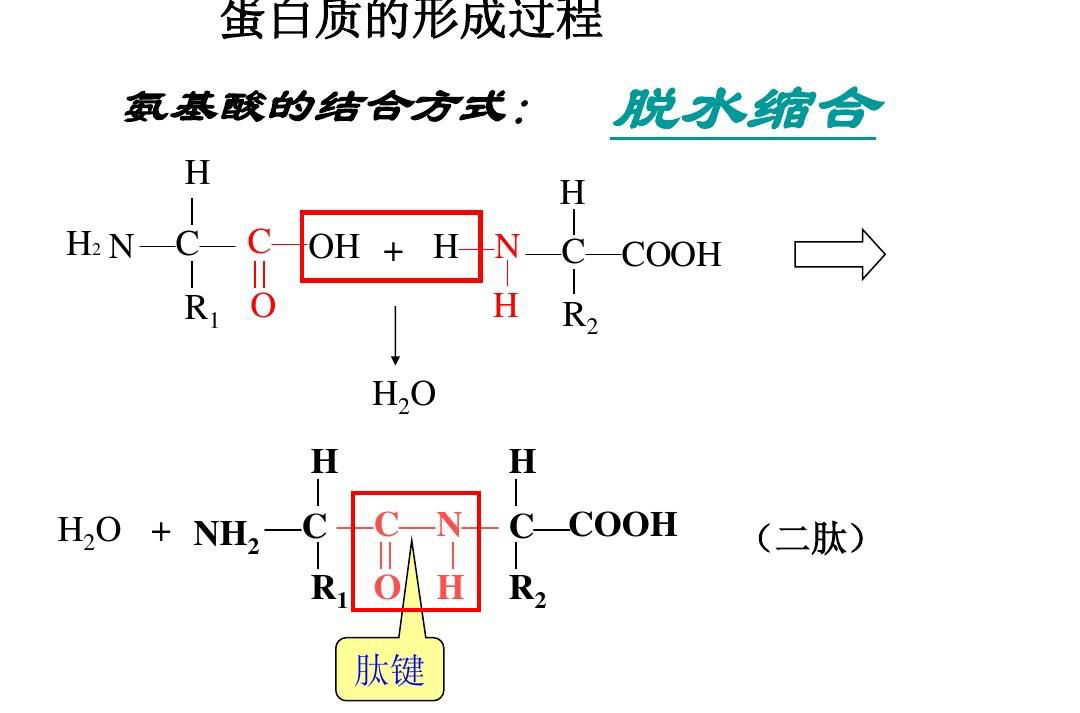
\includegraphics[width=0.7\textwidth]{../images/dehydration-condensation.png}
	\caption{脱水缩合}
	\label{}
\end{figure}

\paragraph{肽键} 是一分子氨基酸的$\alpha$-羧基和一分子氨基酸的$\alpha$-氨基脱水缩合形成的酰胺键,即$-CO-NH-$。

\paragraph{肽链(peptide chain)} 每两个氨基酸相互连接形成一个肽键,多个氨基酸相互连接就形成了多个肽键,由多个氨基酸相互连接形成的含有多个肽键的一条链状结构称为肽链。

\paragraph{蛋白质} 是由氨基酸以“脱水缩合”的方式组成的多肽链经过盘曲折叠形成的具有一定空间结构的物质。蛋白质是由一条或多条多肽链组成的生物大分子,每一条多肽链有二十至数百个氨基酸残基(-R)不等;各种氨基酸残基按一定的顺序排列。蛋白质的氨基酸序列是由对应基因所编码。除了遗传密码所编码的20种基本氨基酸,在蛋白质中,某些氨基酸残基还可以被翻译后修饰而发生化学结构的变化,从而对蛋白质进行激活或调控。多个蛋白质可以一起,往往是通过结合在一起形成稳定的蛋白质复合物,折叠或螺旋构成一定的空间结构,从而发挥某一特定功能。


\paragraph{蛋白质的结构} 蛋白质分子上氨基酸的序列和由此形成的立体结构构成了蛋白质结构的多样性。蛋白质具有一级、二级、三级、四级结构,蛋白质分子的结构决定了它的功能。
\subparagraph{一级结构(primary structure)} 氨基酸残基在蛋白质肽链中的排列顺序称为蛋白质的一级结构,每种蛋白质都有唯一而确切的氨基酸序列。
\subparagraph{二级结构(secondary structure)} 蛋白质分子中肽链并非直链状,而是按一定的规律卷曲(如$\alpha$-螺旋结构)或折叠(如$\beta$-折叠结构)形成特定的空间结构,这是蛋白质的二级结构。蛋白质的二级结构主要依靠肽链中氨基酸残基亚氨基(—NH—)上的氢原子和羰基上的氧原子之间形成的氢键而实现的。
\subparagraph{三级结构(tertiary structure)} 在二级结构的基础上,肽链还按照一定的空间结构进一步形成更复杂的三级结构。肌红蛋白,血红蛋白等正是通过这种结构使其表面的空穴恰好容纳一个血红素分子。
\subparagraph{四级结构(quaternary structure)} 具有三级结构的多肽链按一定空间排列方式结合在一起形成的聚集体结构称为蛋白质的四级结构。如血红蛋白由4个具有三级结构的多肽链构成,其中两个是$\alpha$-链,另两个是$\beta$-链,其四级结构近似椭球形状。















\bibliographystyle{ieeepes}
\bibliography{../Saliency}
\end{document}



























































